%!TEX root = ../../report.tex

\subsection{L-Systems} % (fold)
\label{ssub:l_systems}

Lindenmayer Systems (L-Systems) are a class of string rewriting mechanisms, originally developed by Lindenmayer as a mathematical theory for plant development.

One L-System is a type of a formal grammar and a string rewriting system that is capable of describe the behavior of plant cells and model the growth processes of plant development.

It consists of two different parts, one axiom and a set of production rules. The axiom is the starting point of the system, acting as a seed. Then it is applied in this seed the set of production rules, that change the initial string and producing other strings.
This is an iterative process, so after the production of a larger set of strings, the rules can be applied to each one of them which grows the size of the set even more.

This L-Systems are used to produce natural growth of vegetation (Figure~\ref{fig:trees}), and the generation of Fractals. 


\begin{figure}[htbp]
    \centering
    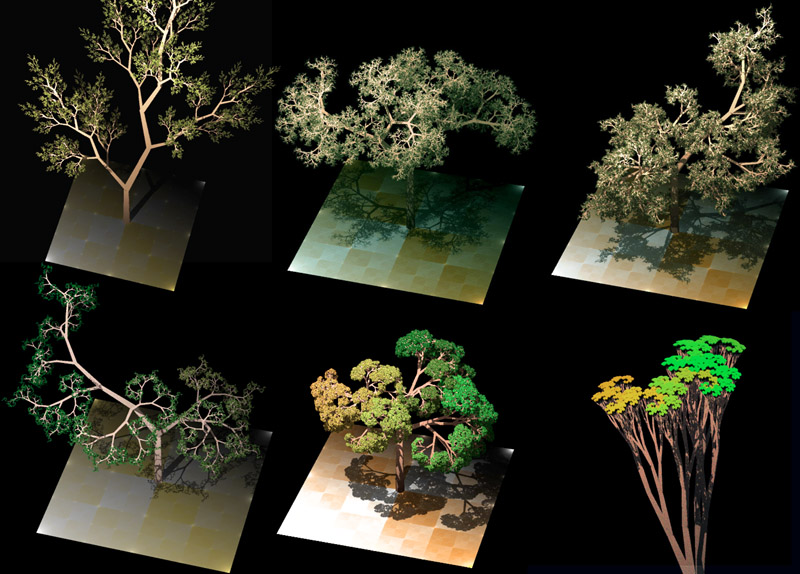
\includegraphics[width=0.95\textwidth]{img/Theory/L_Systems/Dragon_trees.jpg}
    \caption{Trees with L-Systems}
    \label{fig:trees}
\end{figure}


In this process, each symbol is associated with a production rule. For instance having $\{F, +, -\}$ for the alphabet and \emph{production} $\{F \rightarrow
 F+F--F+F\}$. From a starting axiom \emph{aba}, and the application of the rules we have:\\
\begin{equation} \label{eq:seed}
F\\
\end{equation}
\begin{equation} \label{eq:step1}
F+F--F+F\\
\end{equation}
\begin{equation} \label{eq:step2}
F+F--F+F \; + \; F+F--F+F \;- \;- \;F+F--F+F \;+ \;F+F--F+F\\
\end{equation}

%\begin{align}
%\begin{split}
%F\\
%F+F--F+F\\
%F+F--F+F \; + \; F+F--F+F \;- \;- \;F+F--F+F \;+ \;F+F--F+F\\
%\end{split}
%\end{align}
%\\

This is an example of the evolution of one system where the production is applied  in (\ref{eq:seed}) that turns into $F+F--F+F$. In Note that the space between the symbols are just for readability.

All the symbols are assigned with a geometric meaning. The notion of a turtle with a pen, as proposed in \cite{abelson1982aa}, with the symbols being interpreted as moving instructions to the turtle, is a simple way to understand. If ``F'' means forward and the symbols ``+'' and ``-'' are interpreted as rotations counter-clockwise and clockwise respectively by a predefined angle. 

Using the given example, and setting the angle for the rotation to $60^{\circ}$ the result is Figure~\ref{fig:kockLS}.
%$\bigodot \; \bigodot$

\begin{figure}[htbp]
   \centering
   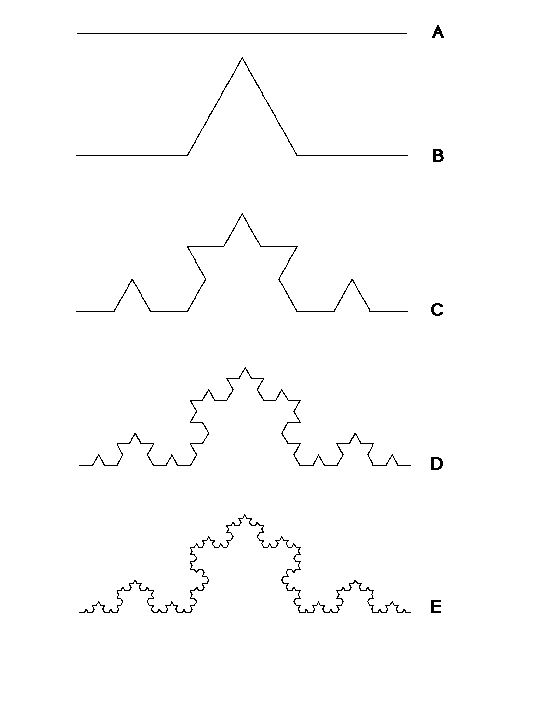
\includegraphics[width=0.75\textwidth]{img/Theory/L_Systems/koch.png}
   \caption{}
   \label{fig:kockLS}
\end{figure}


% This concept of the turtle can be considered also in 3D.



% subsection l_systems (end)